% Options for packages loaded elsewhere
\PassOptionsToPackage{unicode}{hyperref}
\PassOptionsToPackage{hyphens}{url}
%
\documentclass[
]{article}
\usepackage{lmodern}
\usepackage{amssymb,amsmath}
\usepackage{ifxetex,ifluatex}
\ifnum 0\ifxetex 1\fi\ifluatex 1\fi=0 % if pdftex
  \usepackage[T1]{fontenc}
  \usepackage[utf8]{inputenc}
  \usepackage{textcomp} % provide euro and other symbols
\else % if luatex or xetex
  \usepackage{unicode-math}
  \defaultfontfeatures{Scale=MatchLowercase}
  \defaultfontfeatures[\rmfamily]{Ligatures=TeX,Scale=1}
\fi
% Use upquote if available, for straight quotes in verbatim environments
\IfFileExists{upquote.sty}{\usepackage{upquote}}{}
\IfFileExists{microtype.sty}{% use microtype if available
  \usepackage[]{microtype}
  \UseMicrotypeSet[protrusion]{basicmath} % disable protrusion for tt fonts
}{}
\makeatletter
\@ifundefined{KOMAClassName}{% if non-KOMA class
  \IfFileExists{parskip.sty}{%
    \usepackage{parskip}
  }{% else
    \setlength{\parindent}{0pt}
    \setlength{\parskip}{6pt plus 2pt minus 1pt}}
}{% if KOMA class
  \KOMAoptions{parskip=half}}
\makeatother
\usepackage{xcolor}
\IfFileExists{xurl.sty}{\usepackage{xurl}}{} % add URL line breaks if available
\IfFileExists{bookmark.sty}{\usepackage{bookmark}}{\usepackage{hyperref}}
\hypersetup{
  pdftitle={Interpretable Machine Learning Scope Definition Report},
  pdfauthor={Xuan-Son Trinh; Victor Tuekam},
  hidelinks,
  pdfcreator={LaTeX via pandoc}}
\urlstyle{same} % disable monospaced font for URLs
\usepackage[margin=1in]{geometry}
\usepackage{color}
\usepackage{fancyvrb}
\newcommand{\VerbBar}{|}
\newcommand{\VERB}{\Verb[commandchars=\\\{\}]}
\DefineVerbatimEnvironment{Highlighting}{Verbatim}{commandchars=\\\{\}}
% Add ',fontsize=\small' for more characters per line
\usepackage{framed}
\definecolor{shadecolor}{RGB}{248,248,248}
\newenvironment{Shaded}{\begin{snugshade}}{\end{snugshade}}
\newcommand{\AlertTok}[1]{\textcolor[rgb]{0.94,0.16,0.16}{#1}}
\newcommand{\AnnotationTok}[1]{\textcolor[rgb]{0.56,0.35,0.01}{\textbf{\textit{#1}}}}
\newcommand{\AttributeTok}[1]{\textcolor[rgb]{0.77,0.63,0.00}{#1}}
\newcommand{\BaseNTok}[1]{\textcolor[rgb]{0.00,0.00,0.81}{#1}}
\newcommand{\BuiltInTok}[1]{#1}
\newcommand{\CharTok}[1]{\textcolor[rgb]{0.31,0.60,0.02}{#1}}
\newcommand{\CommentTok}[1]{\textcolor[rgb]{0.56,0.35,0.01}{\textit{#1}}}
\newcommand{\CommentVarTok}[1]{\textcolor[rgb]{0.56,0.35,0.01}{\textbf{\textit{#1}}}}
\newcommand{\ConstantTok}[1]{\textcolor[rgb]{0.00,0.00,0.00}{#1}}
\newcommand{\ControlFlowTok}[1]{\textcolor[rgb]{0.13,0.29,0.53}{\textbf{#1}}}
\newcommand{\DataTypeTok}[1]{\textcolor[rgb]{0.13,0.29,0.53}{#1}}
\newcommand{\DecValTok}[1]{\textcolor[rgb]{0.00,0.00,0.81}{#1}}
\newcommand{\DocumentationTok}[1]{\textcolor[rgb]{0.56,0.35,0.01}{\textbf{\textit{#1}}}}
\newcommand{\ErrorTok}[1]{\textcolor[rgb]{0.64,0.00,0.00}{\textbf{#1}}}
\newcommand{\ExtensionTok}[1]{#1}
\newcommand{\FloatTok}[1]{\textcolor[rgb]{0.00,0.00,0.81}{#1}}
\newcommand{\FunctionTok}[1]{\textcolor[rgb]{0.00,0.00,0.00}{#1}}
\newcommand{\ImportTok}[1]{#1}
\newcommand{\InformationTok}[1]{\textcolor[rgb]{0.56,0.35,0.01}{\textbf{\textit{#1}}}}
\newcommand{\KeywordTok}[1]{\textcolor[rgb]{0.13,0.29,0.53}{\textbf{#1}}}
\newcommand{\NormalTok}[1]{#1}
\newcommand{\OperatorTok}[1]{\textcolor[rgb]{0.81,0.36,0.00}{\textbf{#1}}}
\newcommand{\OtherTok}[1]{\textcolor[rgb]{0.56,0.35,0.01}{#1}}
\newcommand{\PreprocessorTok}[1]{\textcolor[rgb]{0.56,0.35,0.01}{\textit{#1}}}
\newcommand{\RegionMarkerTok}[1]{#1}
\newcommand{\SpecialCharTok}[1]{\textcolor[rgb]{0.00,0.00,0.00}{#1}}
\newcommand{\SpecialStringTok}[1]{\textcolor[rgb]{0.31,0.60,0.02}{#1}}
\newcommand{\StringTok}[1]{\textcolor[rgb]{0.31,0.60,0.02}{#1}}
\newcommand{\VariableTok}[1]{\textcolor[rgb]{0.00,0.00,0.00}{#1}}
\newcommand{\VerbatimStringTok}[1]{\textcolor[rgb]{0.31,0.60,0.02}{#1}}
\newcommand{\WarningTok}[1]{\textcolor[rgb]{0.56,0.35,0.01}{\textbf{\textit{#1}}}}
\usepackage{longtable,booktabs}
% Correct order of tables after \paragraph or \subparagraph
\usepackage{etoolbox}
\makeatletter
\patchcmd\longtable{\par}{\if@noskipsec\mbox{}\fi\par}{}{}
\makeatother
% Allow footnotes in longtable head/foot
\IfFileExists{footnotehyper.sty}{\usepackage{footnotehyper}}{\usepackage{footnote}}
\makesavenoteenv{longtable}
\usepackage{graphicx,grffile}
\makeatletter
\def\maxwidth{\ifdim\Gin@nat@width>\linewidth\linewidth\else\Gin@nat@width\fi}
\def\maxheight{\ifdim\Gin@nat@height>\textheight\textheight\else\Gin@nat@height\fi}
\makeatother
% Scale images if necessary, so that they will not overflow the page
% margins by default, and it is still possible to overwrite the defaults
% using explicit options in \includegraphics[width, height, ...]{}
\setkeys{Gin}{width=\maxwidth,height=\maxheight,keepaspectratio}
% Set default figure placement to htbp
\makeatletter
\def\fps@figure{htbp}
\makeatother
\setlength{\emergencystretch}{3em} % prevent overfull lines
\providecommand{\tightlist}{%
  \setlength{\itemsep}{0pt}\setlength{\parskip}{0pt}}
\setcounter{secnumdepth}{5}

\title{Interpretable Machine Learning Scope Definition Report}
\author{Xuan-Son Trinh\footnote{Ludwig Maximilian University of Munich, \href{mailto:Son.Trinh@campus.lmu.de}{\nolinkurl{Son.Trinh@campus.lmu.de}}} \and Victor Tuekam\footnote{Ludwig Maximilian University of Munich, \href{mailto:t.victor@campus.lmu.de}{\nolinkurl{t.victor@campus.lmu.de}}}}
\date{}

\begin{document}
\maketitle

\hypertarget{data-set}{%
\section{Data set}\label{data-set}}

For the Seminar we use the South German Credit dataset, available in the UCI Machine learning repository\footnote{\url{https://archive.ics.uci.edu/ml/datasets/South+German+Credit+\%28UPDATE\%29}}.

The data set consists of a 1000 observations together with 21 attributes. The data was collected between 1973 and 1975. The task associated with this data set is the classification of individuals (instances) according to their credit risk (``good'', ``bad'').

\begin{longtable}[]{@{}ll@{}}
\toprule
\begin{minipage}[b]{0.22\columnwidth}\raggedright
Attribute\strut
\end{minipage} & \begin{minipage}[b]{0.72\columnwidth}\raggedright
Description\strut
\end{minipage}\tabularnewline
\midrule
\endhead
\begin{minipage}[t]{0.22\columnwidth}\raggedright
status\strut
\end{minipage} & \begin{minipage}[t]{0.72\columnwidth}\raggedright
Status of the debtor's checking account with the bank\\
(factor with 4 levels: \emph{``no checking account''}, \emph{``\ldots{} \textless{} 0 DM''}, \emph{``0\textless= \ldots{} \textless{} 200 DM''}, \emph{``\ldots{} \textgreater= 200 DM / salary for at least 1 year''})\strut
\end{minipage}\tabularnewline
\begin{minipage}[t]{0.22\columnwidth}\raggedright
duration\strut
\end{minipage} & \begin{minipage}[t]{0.72\columnwidth}\raggedright
Credit duration in months (int)\strut
\end{minipage}\tabularnewline
\begin{minipage}[t]{0.22\columnwidth}\raggedright
credit\_history\strut
\end{minipage} & \begin{minipage}[t]{0.72\columnwidth}\raggedright
History of the compliance with previous or concurrent credit contracts\\
(factor with 5 levels: \emph{``delay in paying off in the past''}, \emph{``critical account/other credits elsewhere''}, \emph{``no credits taken/all credits paid back duly''}, \emph{``existing credits paid back duly till now''}, \emph{``all credits at this bank paid back duly''})\strut
\end{minipage}\tabularnewline
\begin{minipage}[t]{0.22\columnwidth}\raggedright
purpose\strut
\end{minipage} & \begin{minipage}[t]{0.72\columnwidth}\raggedright
Purpose for which the credit is needed\\
(factor with 11 levels: \emph{``others''}, \emph{``car (new)''}, \emph{``car (used)''}, \emph{``furniture/equipment''}, \emph{``radio/television''}, \emph{``domestic appliances''}, \emph{``repairs''}, \emph{``education''}, \emph{``vacation''}, \emph{``retraining''}, \emph{``business''})\strut
\end{minipage}\tabularnewline
\begin{minipage}[t]{0.22\columnwidth}\raggedright
amount\strut
\end{minipage} & \begin{minipage}[t]{0.72\columnwidth}\raggedright
Amount in DM (int)\strut
\end{minipage}\tabularnewline
\begin{minipage}[t]{0.22\columnwidth}\raggedright
savings\strut
\end{minipage} & \begin{minipage}[t]{0.72\columnwidth}\raggedright
Debtor's savings\\
(factor with 5 levels: \emph{``unknown/no savings account''}, \emph{``\ldots{} \textless{} 100 DM''}, \emph{``100 \textless= \ldots{} \textless{} 500 DM''}, \emph{``500 \textless= \ldots{} \textless{} 1000 DM''}, \emph{``\ldots{} \textgreater= 1000 DM''})\strut
\end{minipage}\tabularnewline
\begin{minipage}[t]{0.22\columnwidth}\raggedright
employment\_duration\strut
\end{minipage} & \begin{minipage}[t]{0.72\columnwidth}\raggedright
Duration of debtor's employment with current employer\\
(factor with 5 levels: \emph{``unemployed''}, \emph{``\textless{} 1 yr''}, \emph{``1 \textless= \ldots{} \textless{} 4 yrs''}, \emph{``4 \textless= \ldots{} \textless{} 7 yrs''}, \emph{``\textgreater= 7 yrs''})\strut
\end{minipage}\tabularnewline
\begin{minipage}[t]{0.22\columnwidth}\raggedright
installment\_rate\strut
\end{minipage} & \begin{minipage}[t]{0.72\columnwidth}\raggedright
Credit installments as a percentage of debtor's disposable income\\
(ordered factor with 4 levels: \emph{``\textgreater= 35''} \textless{} \emph{``25 \textless= \ldots{} \textless{} 35''} \textless{} \emph{``20 \textless= \ldots{} \textless{} 25''} \textless{} \emph{``\textless{} 20''})\strut
\end{minipage}\tabularnewline
\begin{minipage}[t]{0.22\columnwidth}\raggedright
personal\_status\_sex\strut
\end{minipage} & \begin{minipage}[t]{0.72\columnwidth}\raggedright
Combined information on sex and marital status\\
(factor with 4 levels: \emph{``male : divorced/separated''}, \emph{``female : non-single or male : single''}, \emph{``male : married/widowed''}, \emph{``female : single''})\strut
\end{minipage}\tabularnewline
\begin{minipage}[t]{0.22\columnwidth}\raggedright
other\_debtors\strut
\end{minipage} & \begin{minipage}[t]{0.72\columnwidth}\raggedright
Is there another debtor or a guarantor for the credit?\\
(factor with 3 levels: \emph{``none''}, \emph{``co-applicant''}, \emph{``guarantor''})\strut
\end{minipage}\tabularnewline
\begin{minipage}[t]{0.22\columnwidth}\raggedright
present\_residence\strut
\end{minipage} & \begin{minipage}[t]{0.72\columnwidth}\raggedright
Length of time (in years) the debtor lives in the present residence\\
(ordered factor with 4 levels: \emph{``\textless{} 1 yr''} \textless{} \emph{``1 \textless= \ldots{} \textless{} 4 yrs''} \textless{} \emph{``4 \textless= \ldots{} \textless{} 7 yrs''} \textless{} \emph{``\textgreater= 7 yrs''})\strut
\end{minipage}\tabularnewline
\begin{minipage}[t]{0.22\columnwidth}\raggedright
property\strut
\end{minipage} & \begin{minipage}[t]{0.72\columnwidth}\raggedright
The debtor's most valuable property\\
(factor with 4 levels: \emph{``unknown / no property''}, \emph{``car or other''}, \emph{``building soc. savings agr./life insurance''}, \emph{``real estate''})\strut
\end{minipage}\tabularnewline
\begin{minipage}[t]{0.22\columnwidth}\raggedright
age\strut
\end{minipage} & \begin{minipage}[t]{0.72\columnwidth}\raggedright
Age in years (int)\strut
\end{minipage}\tabularnewline
\begin{minipage}[t]{0.22\columnwidth}\raggedright
other\_installment\_plans\strut
\end{minipage} & \begin{minipage}[t]{0.72\columnwidth}\raggedright
Installment plans from providers oder than the credit-giving bank\\
(factor with 3 levels: \emph{``bank''}, \emph{``stores''}, \emph{``none''})\strut
\end{minipage}\tabularnewline
\begin{minipage}[t]{0.22\columnwidth}\raggedright
housing\strut
\end{minipage} & \begin{minipage}[t]{0.72\columnwidth}\raggedright
Type of housing the debtor lives in\\
(factor with 3 levels: \emph{``for free''}, \emph{``rent''}, \emph{``own''})\strut
\end{minipage}\tabularnewline
\begin{minipage}[t]{0.22\columnwidth}\raggedright
number\_credits\strut
\end{minipage} & \begin{minipage}[t]{0.72\columnwidth}\raggedright
Number of credits including the current one the debtor has (or had) at this bank\\
(ordered factor with 4 levels: \emph{``1''} \textless{} \emph{``2-3''} \textless{} \emph{``4-5''} \textless{} \emph{``\textgreater= 6''})\strut
\end{minipage}\tabularnewline
\begin{minipage}[t]{0.22\columnwidth}\raggedright
job\strut
\end{minipage} & \begin{minipage}[t]{0.72\columnwidth}\raggedright
Quality of debtor's job\\
(factor with 4 levels: \emph{``unemployed/unskilled - non-resident''}, \emph{``unskilled - resident''}, \emph{``skilled employee/official''}, \emph{``manager/self-empl./highly qualif. employee''})\strut
\end{minipage}\tabularnewline
\begin{minipage}[t]{0.22\columnwidth}\raggedright
people\_liable\strut
\end{minipage} & \begin{minipage}[t]{0.72\columnwidth}\raggedright
Number of persons who financially depend on the debtor (i.e., are entitled to maintenance)\\
(factor with 2 levels: \emph{``3 or more''}, \emph{``0 to 2''})\strut
\end{minipage}\tabularnewline
\begin{minipage}[t]{0.22\columnwidth}\raggedright
telephone\strut
\end{minipage} & \begin{minipage}[t]{0.72\columnwidth}\raggedright
Is there a telephone landline registered on the debtor's name?\\
(factor with 2 levels: \emph{``no''}, \emph{``yes (under customer name)''})\strut
\end{minipage}\tabularnewline
\begin{minipage}[t]{0.22\columnwidth}\raggedright
foreign\_worker\strut
\end{minipage} & \begin{minipage}[t]{0.72\columnwidth}\raggedright
Is the debtor a foreign worker?\\
(factor with 2 levels: \emph{``yes''}, \emph{``no''})\strut
\end{minipage}\tabularnewline
\begin{minipage}[t]{0.22\columnwidth}\raggedright
credit\_risk\strut
\end{minipage} & \begin{minipage}[t]{0.72\columnwidth}\raggedright
Has the credit contract been complied with (good) or not (bad)?\\
(factor with 2 levels: \emph{``bad''}, \emph{``good''})\strut
\end{minipage}\tabularnewline
\bottomrule
\end{longtable}

\newpage

\hypertarget{load-data}{%
\subsection{Load data}\label{load-data}}

\begin{Shaded}
\begin{Highlighting}[]
\KeywordTok{load}\NormalTok{(}\StringTok{"south-german-credit.Rda"}\NormalTok{)}
\NormalTok{task <-}\StringTok{ }\NormalTok{TaskClassif}\OperatorTok{$}\KeywordTok{new}\NormalTok{(}\StringTok{"german-credit"}\NormalTok{, }
                        \DataTypeTok{backend =}\NormalTok{ data, }
                        \DataTypeTok{target =} \StringTok{"credit_risk"}\NormalTok{, }
                        \DataTypeTok{positive =} \StringTok{"good"}\NormalTok{)}
\end{Highlighting}
\end{Shaded}

\begin{Shaded}
\begin{Highlighting}[]
\KeywordTok{summary}\NormalTok{(data)}
\end{Highlighting}
\end{Shaded}

\begin{verbatim}
##                                         status       duration   
##  no checking account                       :274   Min.   : 4.0  
##  ... < 0 DM                                :269   1st Qu.:12.0  
##  0<= ... < 200 DM                          : 63   Median :18.0  
##  ... >= 200 DM / salary for at least 1 year:394   Mean   :20.9  
##                                                   3rd Qu.:24.0  
##                                                   Max.   :72.0  
##                                                                 
##                                      credit_history                purpose   
##  delay in paying off in the past            : 40    furniture/equipment:280  
##  critical account/other credits elsewhere   : 49    others             :234  
##  no credits taken/all credits paid back duly:530    car (used)         :181  
##  existing credits paid back duly till now   : 88    car (new)          :103  
##  all credits at this bank paid back duly    :293    retraining         : 97  
##                                                     repairs            : 50  
##                                                     (Other)            : 55  
##      amount                            savings          employment_duration
##  Min.   :  250   unknown/no savings account:603   unemployed      : 62     
##  1st Qu.: 1366   ... <  100 DM             :103   < 1 yr          :172     
##  Median : 2320   100 <= ... <  500 DM      : 63   1 <= ... < 4 yrs:339     
##  Mean   : 3271   500 <= ... < 1000 DM      : 48   4 <= ... < 7 yrs:174     
##  3rd Qu.: 3972   ... >= 1000 DM            :183   >= 7 yrs        :253     
##  Max.   :18424                                                             
##                                                                            
##        installment_rate                           personal_status_sex
##  >= 35         :136     male : divorced/separated           : 50     
##  25 <= ... < 35:231     female : non-single or male : single:310     
##  20 <= ... < 25:157     male : married/widowed              :548     
##  < 20          :476     female : single                     : 92     
##                                                                      
##                                                                      
##                                                                      
##       other_debtors        present_residence
##  none        :907   < 1 yr          :130    
##  co-applicant: 41   1 <= ... < 4 yrs:308    
##  guarantor   : 52   4 <= ... < 7 yrs:149    
##                     >= 7 yrs        :413    
##                                             
##                                             
##                                             
##                                       property        age       
##  unknown / no property                    :282   Min.   :19.00  
##  car or other                             :232   1st Qu.:27.00  
##  building soc. savings agr./life insurance:332   Median :33.00  
##  real estate                              :154   Mean   :35.54  
##                                                  3rd Qu.:42.00  
##                                                  Max.   :75.00  
##                                                                 
##  other_installment_plans     housing    number_credits
##  bank  :139              for free:179   1   :633      
##  stores: 47              rent    :714   2-3 :333      
##  none  :814              own     :107   4-5 : 28      
##                                         >= 6:  6      
##                                                       
##                                                       
##                                                       
##                                          job        people_liable
##  unemployed/unskilled - non-resident       : 22   3 or more:155  
##  unskilled - resident                      :200   0 to 2   :845  
##  skilled employee/official                 :630                  
##  manager/self-empl./highly qualif. employee:148                  
##                                                                  
##                                                                  
##                                                                  
##                      telephone   foreign_worker credit_risk
##  no                       :596   yes: 37        bad :300   
##  yes (under customer name):404   no :963        good:700   
##                                                            
##                                                            
##                                                            
##                                                            
## 
\end{verbatim}

The data set doesn't have any missing values and requires little preprocessing to fit our model. It can also be pointed out that the data has class-imbalance problem: The number of ``good'' credited people is more than twice the number of ``bad'' credited people (700 to 300).

\hypertarget{fitting-some-models}{%
\section{Fitting some models}\label{fitting-some-models}}

The \texttt{mlr3} package and other packages from the \texttt{mlr3} ecosystem are used to do the modeling.
The fitted and tuned models are:

\begin{itemize}
\tightlist
\item
  Logistic Regression
\item
  Decision Tree
\item
  Random Forest
\item
  Xgboost
\item
  Support Vector machines (with linear, polynomial, and radial kernels)
\end{itemize}

, in which, logistic regression and decision tree are considered as explainable baseline models; random forest, Xgboost and support vector machines with multiple kernel types as blackbox models.

For preprocessing, we do the following:

\begin{itemize}
\tightlist
\item
  Standardize numerical variables by centering them around their mean and scaling them by their root-mean-square.
\item
  One-hot encode factor and ordered-factor variables.
\item
  To account for the class imbalance in the data set, we perform oversampling of the minority class (``bad'' class).
\end{itemize}

\begin{Shaded}
\begin{Highlighting}[]
\CommentTok{# PipeOps}
\NormalTok{fencoder <-}\StringTok{ }\KeywordTok{po}\NormalTok{(}\StringTok{"encode"}\NormalTok{,}
  \DataTypeTok{method =} \StringTok{"one-hot"}\NormalTok{,}
  \DataTypeTok{affect_columns =} \KeywordTok{selector_type}\NormalTok{(}\StringTok{"factor"}\NormalTok{)}
\NormalTok{)}
\NormalTok{ord_to_int <-}\StringTok{ }\KeywordTok{po}\NormalTok{(}\StringTok{"colapply"}\NormalTok{,}
  \DataTypeTok{applicator =}\NormalTok{ as.integer,}
  \DataTypeTok{affect_columns =} \KeywordTok{selector_type}\NormalTok{(}\StringTok{"ordered"}\NormalTok{)}
\NormalTok{)}

\NormalTok{encoder <-}\StringTok{ }\NormalTok{fencoder }\OperatorTok\StringTok{ }\NormalTok{ord_to_int}

\NormalTok{po_over <-}\StringTok{ }\KeywordTok{po}\NormalTok{(}\StringTok{"classbalancing"}\NormalTok{,}
  \DataTypeTok{id =} \StringTok{"oversample"}\NormalTok{, }\DataTypeTok{adjust =} \StringTok{"minor"}\NormalTok{,}
  \DataTypeTok{reference =} \StringTok{"minor"}\NormalTok{, }\DataTypeTok{shuffle =} \OtherTok{FALSE}\NormalTok{, }\DataTypeTok{ratio =} \FloatTok{2.3}
\NormalTok{)}
\NormalTok{threshold <-}\StringTok{ }\KeywordTok{po}\NormalTok{(}\StringTok{"threshold"}\NormalTok{)}
\NormalTok{pos <-}\StringTok{ }\KeywordTok{po}\NormalTok{(}\StringTok{"scale"}\NormalTok{) }\OperatorTok
\StringTok{  }\NormalTok{encoder }\OperatorTok\StringTok{ }\NormalTok{po_over}
\end{Highlighting}
\end{Shaded}

\hypertarget{tuning-and-benchmarking}{%
\subsection{Tuning and Benchmarking}\label{tuning-and-benchmarking}}

The parameter tuning is done with the following settings for all models. The tuning code is available in the \texttt{.Rmd} source file.

\begin{Shaded}
\begin{Highlighting}[]
\CommentTok{# tuning settings}
\NormalTok{inner_cv5 <-}\StringTok{ }\KeywordTok{rsmp}\NormalTok{(}\StringTok{"cv"}\NormalTok{, }\DataTypeTok{folds =}\NormalTok{ 5L)}
\NormalTok{measure <-}\StringTok{ }\KeywordTok{msr}\NormalTok{(}\StringTok{"classif.bacc"}\NormalTok{)}
\NormalTok{tuner <-}\StringTok{ }\KeywordTok{tnr}\NormalTok{(}\StringTok{"grid_search"}\NormalTok{, }\DataTypeTok{resolution =}\NormalTok{ 7L)}
\NormalTok{terminator <-}\StringTok{ }\KeywordTok{trm}\NormalTok{(}\StringTok{"evals"}\NormalTok{, }\DataTypeTok{n_evals =} \DecValTok{20}\NormalTok{)}
\end{Highlighting}
\end{Shaded}

\begin{Shaded}
\begin{Highlighting}[]
\CommentTok{# Logistic regression}
\NormalTok{log_reg_learner <-}\StringTok{ }\KeywordTok{lrn}\NormalTok{(}\StringTok{"classif.log_reg"}\NormalTok{, }\DataTypeTok{predict_type =} \StringTok{"prob"}\NormalTok{)}
\NormalTok{log_reg_pipeline <-}\StringTok{ }\NormalTok{pos }\OperatorTok\StringTok{ }\NormalTok{log_reg_learner }\OperatorTok\StringTok{ }\NormalTok{threshold}
\NormalTok{log_reg_glearner <-}\StringTok{ }\NormalTok{GraphLearner}\OperatorTok{$}\KeywordTok{new}\NormalTok{(log_reg_pipeline, }\DataTypeTok{id =} \StringTok{"log_reg"}\NormalTok{)}

\NormalTok{log_reg_at <-}\StringTok{ }\NormalTok{AutoTuner}\OperatorTok{$}\KeywordTok{new}\NormalTok{(}
  \DataTypeTok{learner =}\NormalTok{ log_reg_glearner,}
  \DataTypeTok{resampling =}\NormalTok{ inner_cv5,}
  \DataTypeTok{measure =}\NormalTok{ measure,}
  \DataTypeTok{search_space =}\NormalTok{ ParamSet}\OperatorTok{$}\KeywordTok{new}\NormalTok{(}\KeywordTok{list}\NormalTok{(ParamDbl}\OperatorTok{$}\KeywordTok{new}\NormalTok{(}\StringTok{"threshold.thresholds"}\NormalTok{,}
    \DataTypeTok{lower =} \DecValTok{0}\NormalTok{, }\DataTypeTok{upper =} \DecValTok{1}
\NormalTok{  ))),}
  \DataTypeTok{terminator =}\NormalTok{ terminator,}
  \DataTypeTok{tuner =}\NormalTok{ tuner}
\NormalTok{)}

\CommentTok{# Regression trees}
\NormalTok{rpart_learner <-}\StringTok{ }\KeywordTok{lrn}\NormalTok{(}\StringTok{"classif.rpart"}\NormalTok{, }\DataTypeTok{predict_type =} \StringTok{"prob"}\NormalTok{)}
\NormalTok{rpart_pipeline <-}\StringTok{ }\NormalTok{pos }\OperatorTok\StringTok{ }\NormalTok{rpart_learner }\OperatorTok\StringTok{ }\NormalTok{threshold}
\NormalTok{rpart_glearner <-}\StringTok{ }\NormalTok{GraphLearner}\OperatorTok{$}\KeywordTok{new}\NormalTok{(rpart_pipeline, }\DataTypeTok{id =} \StringTok{"rpart"}\NormalTok{)}

\NormalTok{rpart_at <-}\StringTok{ }\NormalTok{AutoTuner}\OperatorTok{$}\KeywordTok{new}\NormalTok{(}
  \DataTypeTok{learner =}\NormalTok{ rpart_glearner,}
  \DataTypeTok{resampling =}\NormalTok{ inner_cv5,}
  \DataTypeTok{measure =}\NormalTok{ measure,}
  \DataTypeTok{search_space =}\NormalTok{ ParamSet}\OperatorTok{$}\KeywordTok{new}\NormalTok{(}\KeywordTok{list}\NormalTok{(ParamDbl}\OperatorTok{$}\KeywordTok{new}\NormalTok{(}\StringTok{"threshold.thresholds"}\NormalTok{,}
    \DataTypeTok{lower =} \DecValTok{0}\NormalTok{, }\DataTypeTok{upper =} \DecValTok{1}
\NormalTok{  ))),}
  \DataTypeTok{terminator =}\NormalTok{ terminator,}
  \DataTypeTok{tuner =}\NormalTok{ tuner}
\NormalTok{)}

\CommentTok{# Random forest}
\NormalTok{ranger_pipeline <-}\StringTok{ }\NormalTok{pos }\OperatorTok\StringTok{ }\KeywordTok{lrn}\NormalTok{(}\StringTok{"classif.ranger"}\NormalTok{,}
  \DataTypeTok{predict_type =} \StringTok{"prob"}
\NormalTok{) }\OperatorTok\StringTok{ }\NormalTok{threshold}
\NormalTok{ranger_glearner <-}\StringTok{ }\NormalTok{GraphLearner}\OperatorTok{$}\KeywordTok{new}\NormalTok{(ranger_pipeline, }\DataTypeTok{id =} \StringTok{"ranger"}\NormalTok{)}

\NormalTok{ranger_tune_ps <-}\StringTok{ }\NormalTok{ParamSet}\OperatorTok{$}\KeywordTok{new}\NormalTok{(}\KeywordTok{list}\NormalTok{(}
\NormalTok{  ParamDbl}\OperatorTok{$}\KeywordTok{new}\NormalTok{(}\StringTok{"threshold.thresholds"}\NormalTok{, }\DataTypeTok{lower =} \DecValTok{0}\NormalTok{, }\DataTypeTok{upper =} \DecValTok{1}\NormalTok{),}
\NormalTok{  ParamInt}\OperatorTok{$}\KeywordTok{new}\NormalTok{(}\StringTok{"classif.ranger.num.trees"}\NormalTok{,}
    \DataTypeTok{lower =} \DecValTok{100}\NormalTok{, }\DataTypeTok{upper =} \DecValTok{140}
\NormalTok{  ), }\CommentTok{# number of trees}
\NormalTok{  ParamInt}\OperatorTok{$}\KeywordTok{new}\NormalTok{(}\StringTok{"classif.ranger.mtry"}\NormalTok{,}
    \DataTypeTok{lower =} \DecValTok{1}\NormalTok{, }\DataTypeTok{upper =} \KeywordTok{ceiling}\NormalTok{(task}\OperatorTok{$}\NormalTok{ncol }\OperatorTok{/}\StringTok{ }\DecValTok{2}\NormalTok{)}
\NormalTok{  ), }\CommentTok{# number of variables to possibly split at in each node}
\NormalTok{  ParamInt}\OperatorTok{$}\KeywordTok{new}\NormalTok{(}\StringTok{"classif.ranger.max.depth"}\NormalTok{,}
    \DataTypeTok{lower =} \DecValTok{2}\NormalTok{, }\DataTypeTok{upper =} \DecValTok{20}
\NormalTok{  ) }\CommentTok{# maximum depth of the tree}
\NormalTok{))}

\NormalTok{ranger_at <-}\StringTok{ }\NormalTok{AutoTuner}\OperatorTok{$}\KeywordTok{new}\NormalTok{(}
  \DataTypeTok{learner =}\NormalTok{ ranger_glearner,}
  \DataTypeTok{resampling =}\NormalTok{ inner_cv5,}
  \DataTypeTok{measure =}\NormalTok{ measure,}
  \DataTypeTok{search_space =}\NormalTok{ ranger_tune_ps,}
  \DataTypeTok{terminator =}\NormalTok{ terminator,}
  \DataTypeTok{tuner =}\NormalTok{ tuner}
\NormalTok{)}

\CommentTok{# Svms}
\NormalTok{linear_svm_learner <-}\StringTok{ }\KeywordTok{lrn}\NormalTok{(}\StringTok{"classif.svm"}\NormalTok{,}
  \DataTypeTok{type =} \StringTok{"C-classification"}\NormalTok{, }\DataTypeTok{kernel =} \StringTok{"linear"}\NormalTok{,}
  \DataTypeTok{predict_type =} \StringTok{"prob"}
\NormalTok{)}
\NormalTok{poly_svm_learner <-}\StringTok{ }\KeywordTok{lrn}\NormalTok{(}\StringTok{"classif.svm"}\NormalTok{,}
  \DataTypeTok{type =} \StringTok{"C-classification"}\NormalTok{, }\DataTypeTok{kernel =} \StringTok{"polynomial"}\NormalTok{,}
  \DataTypeTok{predict_type =} \StringTok{"prob"}
\NormalTok{)}
\NormalTok{radial_svm_learner <-}\StringTok{ }\KeywordTok{lrn}\NormalTok{(}\StringTok{"classif.svm"}\NormalTok{,}
  \DataTypeTok{type =} \StringTok{"C-classification"}\NormalTok{, }\DataTypeTok{kernel =} \StringTok{"radial"}\NormalTok{,}
  \DataTypeTok{predict_type =} \StringTok{"prob"}
\NormalTok{)}

\CommentTok{# Pipelines}
\NormalTok{linear_svm_pipeline <-}\StringTok{ }\NormalTok{pos }\OperatorTok\StringTok{ }\NormalTok{linear_svm_learner }\OperatorTok\StringTok{ }\NormalTok{threshold}
\NormalTok{poly_svm_pipeline <-}\StringTok{ }\NormalTok{pos }\OperatorTok\StringTok{ }\NormalTok{poly_svm_learner }\OperatorTok\StringTok{ }\NormalTok{threshold}
\NormalTok{radial_svm_pipeline <-}\StringTok{ }\NormalTok{pos }\OperatorTok\StringTok{ }\NormalTok{radial_svm_learner }\OperatorTok\StringTok{ }\NormalTok{threshold}

\CommentTok{# Learners}
\NormalTok{linear_svm_glearner <-}\StringTok{ }\NormalTok{GraphLearner}\OperatorTok{$}\KeywordTok{new}\NormalTok{(linear_svm_pipeline, }\DataTypeTok{id =} \StringTok{"linear_svm"}\NormalTok{)}
\NormalTok{poly_svm_glearner <-}\StringTok{ }\NormalTok{GraphLearner}\OperatorTok{$}\KeywordTok{new}\NormalTok{(poly_svm_pipeline, }\DataTypeTok{id =} \StringTok{"poly_svm"}\NormalTok{)}
\NormalTok{radial_svm_glearner <-}\StringTok{ }\NormalTok{GraphLearner}\OperatorTok{$}\KeywordTok{new}\NormalTok{(radial_svm_pipeline, }\DataTypeTok{id =} \StringTok{"radial_svm"}\NormalTok{)}

\CommentTok{# Search spaces}
\NormalTok{poly_svm_search_space <-}\StringTok{ }\NormalTok{ParamSet}\OperatorTok{$}\KeywordTok{new}\NormalTok{(}\KeywordTok{list}\NormalTok{(}
\NormalTok{  ParamDbl}\OperatorTok{$}\KeywordTok{new}\NormalTok{(}\StringTok{"threshold.thresholds"}\NormalTok{, }\DataTypeTok{lower =} \DecValTok{0}\NormalTok{, }\DataTypeTok{upper =} \DecValTok{1}\NormalTok{),}
\NormalTok{  ParamDbl}\OperatorTok{$}\KeywordTok{new}\NormalTok{(}\StringTok{"classif.svm.cost"}\NormalTok{, }\DataTypeTok{lower =} \FloatTok{0.01}\NormalTok{, }\DataTypeTok{upper =} \DecValTok{100}\NormalTok{),}
\NormalTok{  ParamDbl}\OperatorTok{$}\KeywordTok{new}\NormalTok{(}\StringTok{"classif.svm.gamma"}\NormalTok{, }\DataTypeTok{lower =} \FloatTok{0.0001}\NormalTok{, }\DataTypeTok{upper =} \DecValTok{1}\NormalTok{),}
\NormalTok{  ParamInt}\OperatorTok{$}\KeywordTok{new}\NormalTok{(}\StringTok{"classif.svm.degree"}\NormalTok{, }\DataTypeTok{lower =} \DecValTok{1}\NormalTok{, }\DataTypeTok{upper =} \DecValTok{4}\NormalTok{)}
\NormalTok{))}

\NormalTok{radial_svm_search_space <-}\StringTok{ }\NormalTok{ParamSet}\OperatorTok{$}\KeywordTok{new}\NormalTok{(}\KeywordTok{list}\NormalTok{(}
\NormalTok{  ParamDbl}\OperatorTok{$}\KeywordTok{new}\NormalTok{(}\StringTok{"threshold.thresholds"}\NormalTok{, }\DataTypeTok{lower =} \DecValTok{0}\NormalTok{, }\DataTypeTok{upper =} \DecValTok{1}\NormalTok{),}
\NormalTok{  ParamDbl}\OperatorTok{$}\KeywordTok{new}\NormalTok{(}\StringTok{"classif.svm.cost"}\NormalTok{, }\DataTypeTok{lower =} \FloatTok{0.01}\NormalTok{, }\DataTypeTok{upper =} \DecValTok{100}\NormalTok{),}
\NormalTok{  ParamDbl}\OperatorTok{$}\KeywordTok{new}\NormalTok{(}\StringTok{"classif.svm.gamma"}\NormalTok{, }\DataTypeTok{lower =} \FloatTok{0.0001}\NormalTok{, }\DataTypeTok{upper =} \DecValTok{1}\NormalTok{)}
\NormalTok{))}

\NormalTok{linear_svm_search_space <-}\StringTok{ }\NormalTok{ParamSet}\OperatorTok{$}\KeywordTok{new}\NormalTok{(}\KeywordTok{list}\NormalTok{(}
\NormalTok{  ParamDbl}\OperatorTok{$}\KeywordTok{new}\NormalTok{(}\StringTok{"threshold.thresholds"}\NormalTok{, }\DataTypeTok{lower =} \DecValTok{0}\NormalTok{, }\DataTypeTok{upper =} \DecValTok{1}\NormalTok{),}
\NormalTok{  ParamDbl}\OperatorTok{$}\KeywordTok{new}\NormalTok{(}\StringTok{"classif.svm.cost"}\NormalTok{, }\DataTypeTok{lower =} \FloatTok{0.01}\NormalTok{, }\DataTypeTok{upper =} \DecValTok{100}\NormalTok{)}
\NormalTok{))}

\NormalTok{linear_svm_at <-}\StringTok{ }\NormalTok{AutoTuner}\OperatorTok{$}\KeywordTok{new}\NormalTok{(}
  \DataTypeTok{learner =}\NormalTok{ linear_svm_glearner,}
  \DataTypeTok{resampling =}\NormalTok{ inner_cv5,}
  \DataTypeTok{terminator =}\NormalTok{ terminator,}
  \DataTypeTok{search_space =}\NormalTok{ linear_svm_search_space,}
  \DataTypeTok{tuner =}\NormalTok{ tuner,}
  \DataTypeTok{measure =}\NormalTok{ measure}
\NormalTok{)}
\NormalTok{poly_svm_at <-}\StringTok{ }\NormalTok{AutoTuner}\OperatorTok{$}\KeywordTok{new}\NormalTok{(}
  \DataTypeTok{learner =}\NormalTok{ poly_svm_glearner,}
  \DataTypeTok{resampling =}\NormalTok{ inner_cv5,}
  \DataTypeTok{terminator =}\NormalTok{ terminator,}
  \DataTypeTok{search_space =}\NormalTok{ poly_svm_search_space,}
  \DataTypeTok{tuner =}\NormalTok{ tuner,}
  \DataTypeTok{measure =}\NormalTok{ measure}
\NormalTok{)}
\NormalTok{radial_svm_at <-}\StringTok{ }\NormalTok{AutoTuner}\OperatorTok{$}\KeywordTok{new}\NormalTok{(}
  \DataTypeTok{learner =}\NormalTok{ radial_svm_glearner,}
  \DataTypeTok{resampling =}\NormalTok{ inner_cv5,}
  \DataTypeTok{terminator =}\NormalTok{ terminator,}
  \DataTypeTok{search_space =}\NormalTok{ radial_svm_search_space,}
  \DataTypeTok{tuner =}\NormalTok{ tuner,}
  \DataTypeTok{measure =}\NormalTok{ measure}
\NormalTok{)}
\end{Highlighting}
\end{Shaded}

\begin{Shaded}
\begin{Highlighting}[]
\KeywordTok{autoplot}\NormalTok{(bmr, }\DataTypeTok{measure =} \KeywordTok{msr}\NormalTok{(}\StringTok{"classif.fbeta"}\NormalTok{)) }\OperatorTok{+}
\StringTok{  }\KeywordTok{theme}\NormalTok{(}\DataTypeTok{axis.text.x =} \KeywordTok{element_text}\NormalTok{(}\DataTypeTok{angle =} \DecValTok{45}\NormalTok{, }\DataTypeTok{hjust =} \DecValTok{1}\NormalTok{))}
\end{Highlighting}
\end{Shaded}

\begin{figure}

{\centering 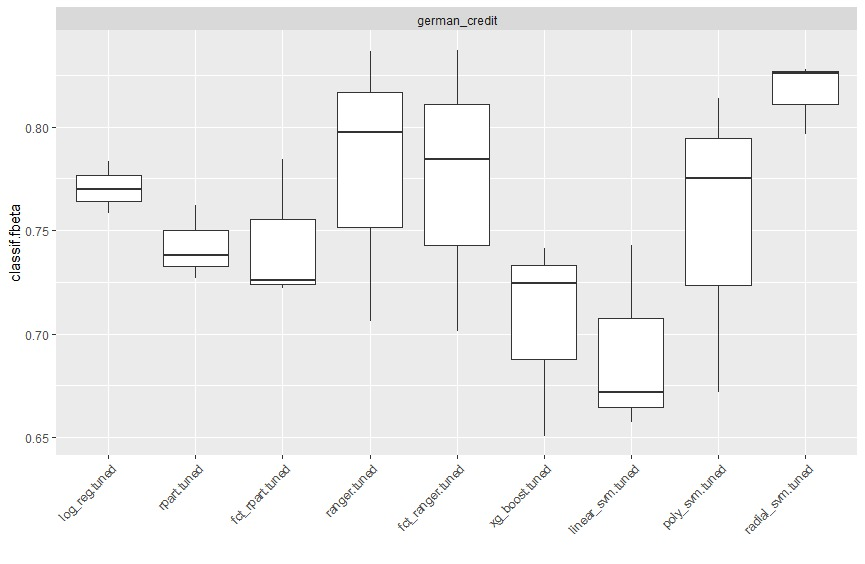
\includegraphics[width=0.8\linewidth]{plots/fbeta} 

}

\caption{Evaluation}\label{fig:evaluation-results}
\end{figure}

As can be seen from the Figure \ref{fig:evaluation-results}, the tuned SVM using radial basis kernel has the best performance (highest F1 score) and therefore is used for subsequent interpretations. We also observe that the performace of tree based models doesn't change significantly, when categorical variables are not coverted to numerics (See box plots in Figure labeled \texttt{fct\_}).

\begin{Shaded}
\begin{Highlighting}[]
\NormalTok{radial_svm_at}\OperatorTok{$}\NormalTok{predict_type =}\StringTok{ "prob"}
\NormalTok{radial_svm_at}\OperatorTok{$}\KeywordTok{train}\NormalTok{(task)}
\end{Highlighting}
\end{Shaded}

\hypertarget{interpretable-machine-learning-methods-and-hypotheses}{%
\section{Interpretable Machine Learning Methods and Hypotheses}\label{interpretable-machine-learning-methods-and-hypotheses}}

We first give a brief description of some interpretable machine learning methods we would use to investigate our hypotheses. The methods are more thoroughly described in the Interpertable Machine Learning book\footnote{\url{https://christophm.github.io/interpretable-ml-book/}}.

\hypertarget{interpretable-machine-learning-methods}{%
\subsection{Interpretable Machine Learning Methods}\label{interpretable-machine-learning-methods}}

\hypertarget{feature-effects}{%
\subsubsection{Feature Effects}\label{feature-effects}}

\textbf{Partial Dependence Plot (PDP):} It shows the marginal effect a feature has on the output of a model.

\textbf{Accumulated Local Effects (ALE) Plots:} A faster and unbiased alternative to PDP. It calculates the differences in predictions instead of averages.

\textbf{SHAP Dependence Plots:} An alternative to PDP to visualize feature effects on the model output.

\textbf{SHAP Summary Plots:} Visualizes feature importance and effects in a single plot.

\hypertarget{global-feature-importance}{%
\subsubsection{Global Feature Importance}\label{global-feature-importance}}

\textbf{Permutation Feature Importance:} It measures the increase in prediction error after permuting the feature values.

\hypertarget{feature-interaction}{%
\subsubsection{Feature Interaction}\label{feature-interaction}}

\textbf{H-Statistic:} Friedman's H-Statistic can tell us two things. (1) Whether and to what extent a feature interacts with all other features in the model and (2) whether and to what extent two features interact with one-another.

\hypertarget{local-interpretation-methods}{%
\subsubsection{Local Interpretation Methods}\label{local-interpretation-methods}}

\textbf{Anchors:} Provides an ``anchor'' explanation of individual model predictions. The ``anchor'' explanation is a decision rule, where-in unaccounted variables do not affect the prediction.

\hypertarget{example-based-explanations}{%
\subsubsection{Example-Based Explanations}\label{example-based-explanations}}

\textbf{Counterfactual Explanations:} A counterfactual explanation of a prediction describes the smallest change to the feature values that changes the prediction to the predefined output.

\hypertarget{hypotheses-and-suggested-iml-methods}{%
\subsection{Hypotheses and Suggested IML Methods}\label{hypotheses-and-suggested-iml-methods}}

To work on this part, we use the IML methods implemented in the package \texttt{iml}

\begin{Shaded}
\begin{Highlighting}[]
\KeywordTok{library}\NormalTok{(iml)}
\end{Highlighting}
\end{Shaded}

\begin{longtable}[]{@{}ll@{}}
\toprule
\begin{minipage}[b]{0.47\columnwidth}\raggedright
Hypothesis\strut
\end{minipage} & \begin{minipage}[b]{0.47\columnwidth}\raggedright
IML Method\strut
\end{minipage}\tabularnewline
\midrule
\endhead
\begin{minipage}[t]{0.47\columnwidth}\raggedright
What are the most important features for the prediction of the \texttt{credit\_risk}\strut
\end{minipage} & \begin{minipage}[t]{0.47\columnwidth}\raggedright
Permutation Featurn Importance\strut
\end{minipage}\tabularnewline
\begin{minipage}[t]{0.47\columnwidth}\raggedright
Having no \texttt{property} should imply a bad \texttt{credit\_risk}\strut
\end{minipage} & \begin{minipage}[t]{0.47\columnwidth}\raggedright
ALE\strut
\end{minipage}\tabularnewline
\begin{minipage}[t]{0.47\columnwidth}\raggedright
Is being older better for \texttt{credit\_risk}\strut
\end{minipage} & \begin{minipage}[t]{0.47\columnwidth}\raggedright
ALE\strut
\end{minipage}\tabularnewline
\begin{minipage}[t]{0.47\columnwidth}\raggedright
Is there an interaction between \texttt{job} and \texttt{credit\_history}? People with delayed \texttt{credit\_history} often have low quality \texttt{job}\strut
\end{minipage} & \begin{minipage}[t]{0.47\columnwidth}\raggedright
H-Statistic\strut
\end{minipage}\tabularnewline
\begin{minipage}[t]{0.47\columnwidth}\raggedright
What is the smallest change in \texttt{number\_credits} that can toggle the model output from \texttt{good} to \texttt{bad}\strut
\end{minipage} & \begin{minipage}[t]{0.47\columnwidth}\raggedright
Counterfactual Explanations\strut
\end{minipage}\tabularnewline
\begin{minipage}[t]{0.47\columnwidth}\raggedright
People with high quality \texttt{job}s have good \texttt{credit\_risk}\strut
\end{minipage} & \begin{minipage}[t]{0.47\columnwidth}\raggedright
SHAP Feature Importance \& SHAP Summary Plots\strut
\end{minipage}\tabularnewline
\begin{minipage}[t]{0.47\columnwidth}\raggedright
How strong is the interaction between each feature and other features in German Credit Dataset?\strut
\end{minipage} & \begin{minipage}[t]{0.47\columnwidth}\raggedright
H-Statistic\strut
\end{minipage}\tabularnewline
\begin{minipage}[t]{0.47\columnwidth}\raggedright
Does having no \texttt{property} mean bad \texttt{credit\_risk} and how does this relate to age\strut
\end{minipage} & \begin{minipage}[t]{0.47\columnwidth}\raggedright
Anchors, H-Statistic\strut
\end{minipage}\tabularnewline
\begin{minipage}[t]{0.47\columnwidth}\raggedright
Being a foreign worker does not affect your credit risk. If this feature is important for prediction, this implies discrimination\strut
\end{minipage} & \begin{minipage}[t]{0.47\columnwidth}\raggedright
Permutation Feature Importance \& ALE\strut
\end{minipage}\tabularnewline
\begin{minipage}[t]{0.47\columnwidth}\raggedright
The better the savings, the better your credit risk\strut
\end{minipage} & \begin{minipage}[t]{0.47\columnwidth}\raggedright
Permutation Feature Importance, SHAP Feature Importance \& SHAP Summary Plots\strut
\end{minipage}\tabularnewline
\begin{minipage}[t]{0.47\columnwidth}\raggedright
How does a change in the \texttt{savings} threshold change the \texttt{credit\_risk}\strut
\end{minipage} & \begin{minipage}[t]{0.47\columnwidth}\raggedright
ALE, Counterfactual Explanations\strut
\end{minipage}\tabularnewline
\begin{minipage}[t]{0.47\columnwidth}\raggedright
The higher the \texttt{installment\_rate} the better the \texttt{credit\_risk}\strut
\end{minipage} & \begin{minipage}[t]{0.47\columnwidth}\raggedright
Partial Dependence Plot, SHAP Dependence Plot \& SHAP Summary Plots\strut
\end{minipage}\tabularnewline
\begin{minipage}[t]{0.47\columnwidth}\raggedright
Does owning a house (\texttt{housing}) mean good \texttt{credit\_risk}\strut
\end{minipage} & \begin{minipage}[t]{0.47\columnwidth}\raggedright
Partial Dependence Plot, SHAP Dependence Plot \& SHAP Summary Plot\strut
\end{minipage}\tabularnewline
\bottomrule
\end{longtable}

\begin{enumerate}
\def\labelenumi{\arabic{enumi}.}
\tightlist
\item
  What are the most important features for the prediction of the \texttt{credit\_risk}?\\
  The importance of features can be uncovered using Permutation Feature Importance (Figure \ref{fig:feature-importance}). Through the increase in the prediction error, we can see that the most important feature for predicting \texttt{credit\_risk} is \texttt{status} of your checking account, which stands out from the other features of the dataset. It is followed by \texttt{duration}, \texttt{purpose}, \texttt{amount}, \texttt{credit\_history}, \texttt{installment\_rate}, etc. with gradual decrease in the importance.
\end{enumerate}

\begin{Shaded}
\begin{Highlighting}[]
\NormalTok{imp <-}\StringTok{ }\NormalTok{FeatureImp}\OperatorTok{$}\KeywordTok{new}\NormalTok{(model, }\DataTypeTok{loss=}\StringTok{"ce"}\NormalTok{)}
\KeywordTok{plot}\NormalTok{(imp)}
\end{Highlighting}
\end{Shaded}

\begin{figure}

{\centering 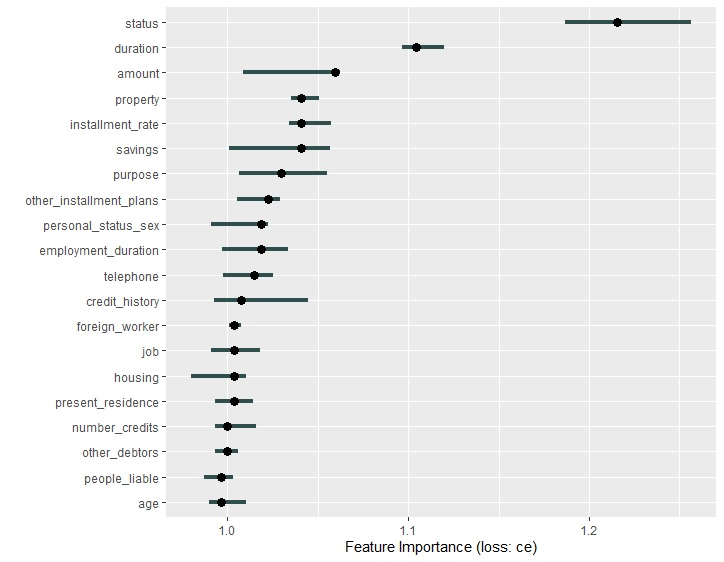
\includegraphics[width=0.8\linewidth]{plots/feature_importance_ce} 

}

\caption{German Credit Feature Importance}\label{fig:feature-importance}
\end{figure}

\begin{enumerate}
\def\labelenumi{\arabic{enumi}.}
\setcounter{enumi}{1}
\item
  Having no \texttt{property} should imply a bad \texttt{credit\_risk}\\
  NaN
\item
  Is being older better for \texttt{credit\_risk}?\\
  To answer this question, we use the ALE plot (Figure \ref{fig:ale-age}). The ALE plot shows a linear relationship between the predicted probability and \texttt{age}. The model confirms that the older we get, the better influence we have on the credit score.
\end{enumerate}

\begin{Shaded}
\begin{Highlighting}[]
\NormalTok{eff <-}\StringTok{ }\NormalTok{FeatureEffect}\OperatorTok{$}\KeywordTok{new}\NormalTok{(model, }\DataTypeTok{feature =} \KeywordTok{c}\NormalTok{(}\StringTok{"age"}\NormalTok{), }\DataTypeTok{method=}\StringTok{'ale'}\NormalTok{)}
\NormalTok{eff}\OperatorTok{$}\KeywordTok{plot}\NormalTok{()}
\end{Highlighting}
\end{Shaded}

\begin{figure}

{\centering 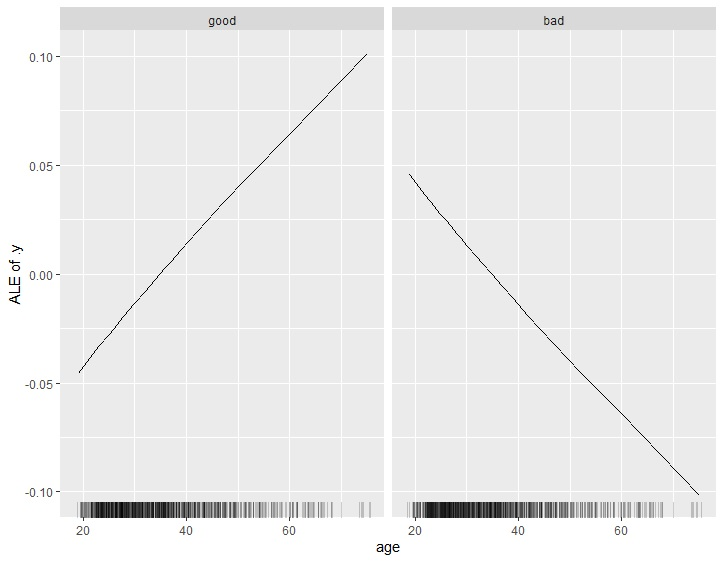
\includegraphics[width=0.8\linewidth]{plots/ale_age} 

}

\caption{ALE Plot of `age`}\label{fig:ale-age}
\end{figure}

\begin{enumerate}
\def\labelenumi{\arabic{enumi}.}
\setcounter{enumi}{3}
\item
  Is there an interaction between \texttt{job} and \texttt{credit\_history}? People with delayed \texttt{credit\_history} often have low quality \texttt{job}\\
  NaN
\item
  What is the smallest change in \texttt{number\_credits} that can toggle the model output from \texttt{good} to \texttt{bad}?\\
  NaN
\item
  People with high quality \texttt{job}s have good \texttt{credit\_risk}\\
  ALE plot continues to be used to answer this question (Figure \ref{fig:ale-job}). According to the plot, being unskilled and non-resident or being manager/high qualified employee causes a loss in your credit score while being skilled employees or just being a resident can have a positive effect on your credit score. This raises some questions for us to think about. Why are both unskilled but
  being resident has good effect on the credit and bad effect otherwise? Is it some kind of discrimination to foreigners? The plot also shows that being a high-qualified employee has the worst effect on the credit, which is an absurd thing. These may be explained due to the fact that the dataset is relatively small so it may possess high variance.
\end{enumerate}

\begin{Shaded}
\begin{Highlighting}[]
\NormalTok{eff <-}\StringTok{ }\NormalTok{FeatureEffect}\OperatorTok{$}\KeywordTok{new}\NormalTok{(model, }\DataTypeTok{feature =} \KeywordTok{c}\NormalTok{(}\StringTok{"job"}\NormalTok{), }\DataTypeTok{method=}\StringTok{'ale'}\NormalTok{)}
\NormalTok{eff}\OperatorTok{$}\KeywordTok{plot}\NormalTok{()}
\end{Highlighting}
\end{Shaded}

\begin{figure}

{\centering 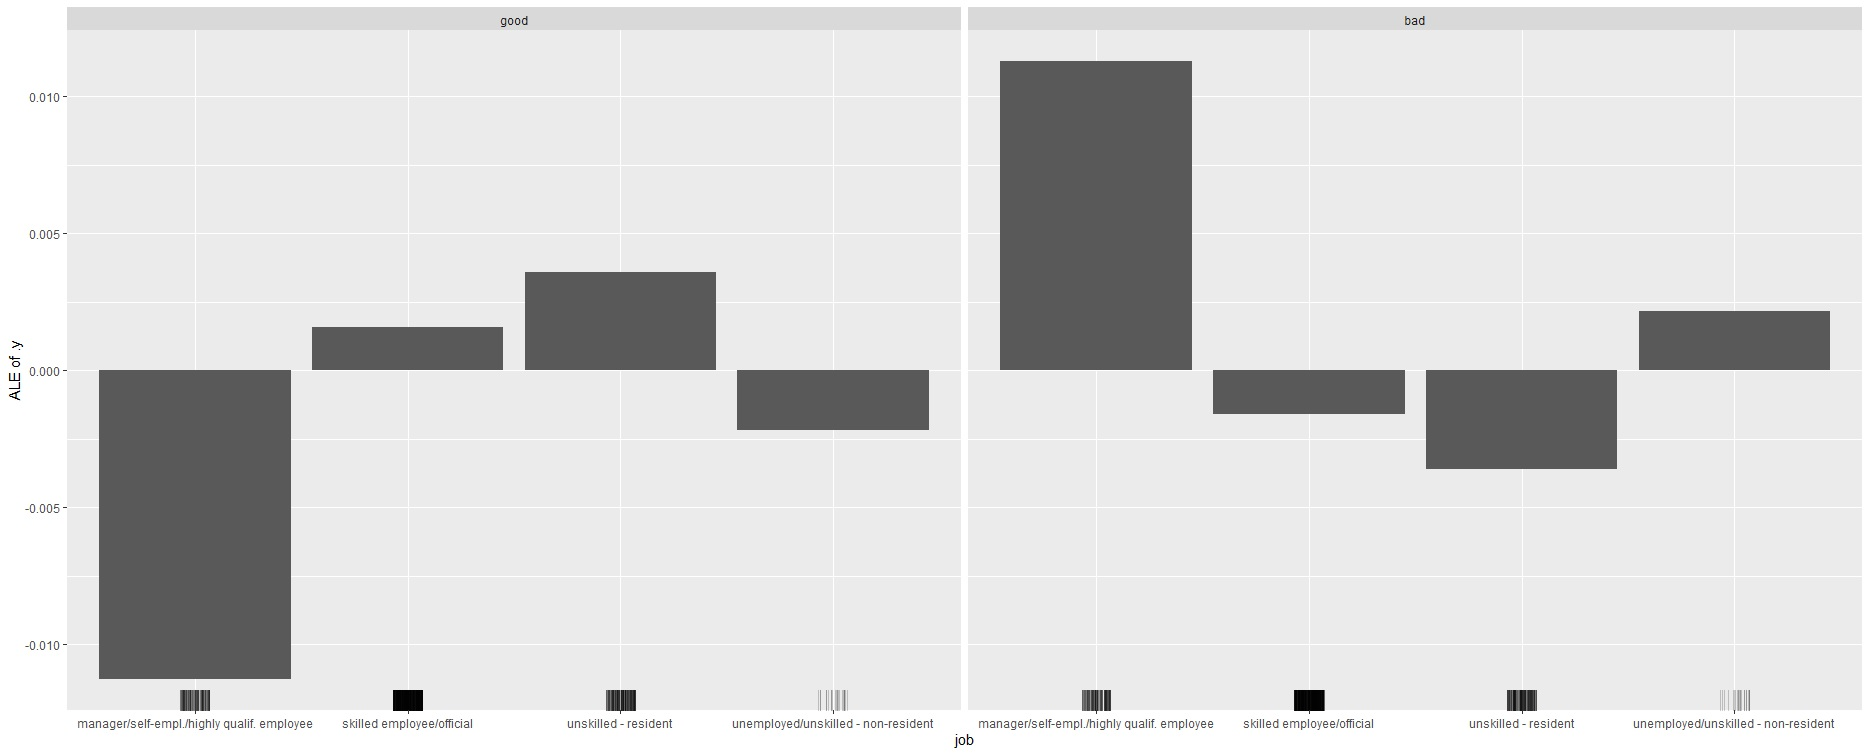
\includegraphics[width=0.8\linewidth]{plots/ale_job} 

}

\caption{ALE Plot of `job`}\label{fig:ale-job}
\end{figure}

\begin{enumerate}
\def\labelenumi{\arabic{enumi}.}
\setcounter{enumi}{6}
\tightlist
\item
  How strong is the interaction between each feature and all other features in German Credit Dataset?\\
  To answer the question, we calculate the H-statistic between each feature and all other features. The result is presented in Figure \ref{fig:interaction}. As can be seen, the interactions are not strong where the highest is just approximately 0.11.
\end{enumerate}

\begin{Shaded}
\begin{Highlighting}[]
\NormalTok{ia <-}\StringTok{ }\NormalTok{Interaction}\OperatorTok{$}\KeywordTok{new}\NormalTok{(model)}
\KeywordTok{plot}\NormalTok{(ia)}
\end{Highlighting}
\end{Shaded}

\begin{figure}

{\centering 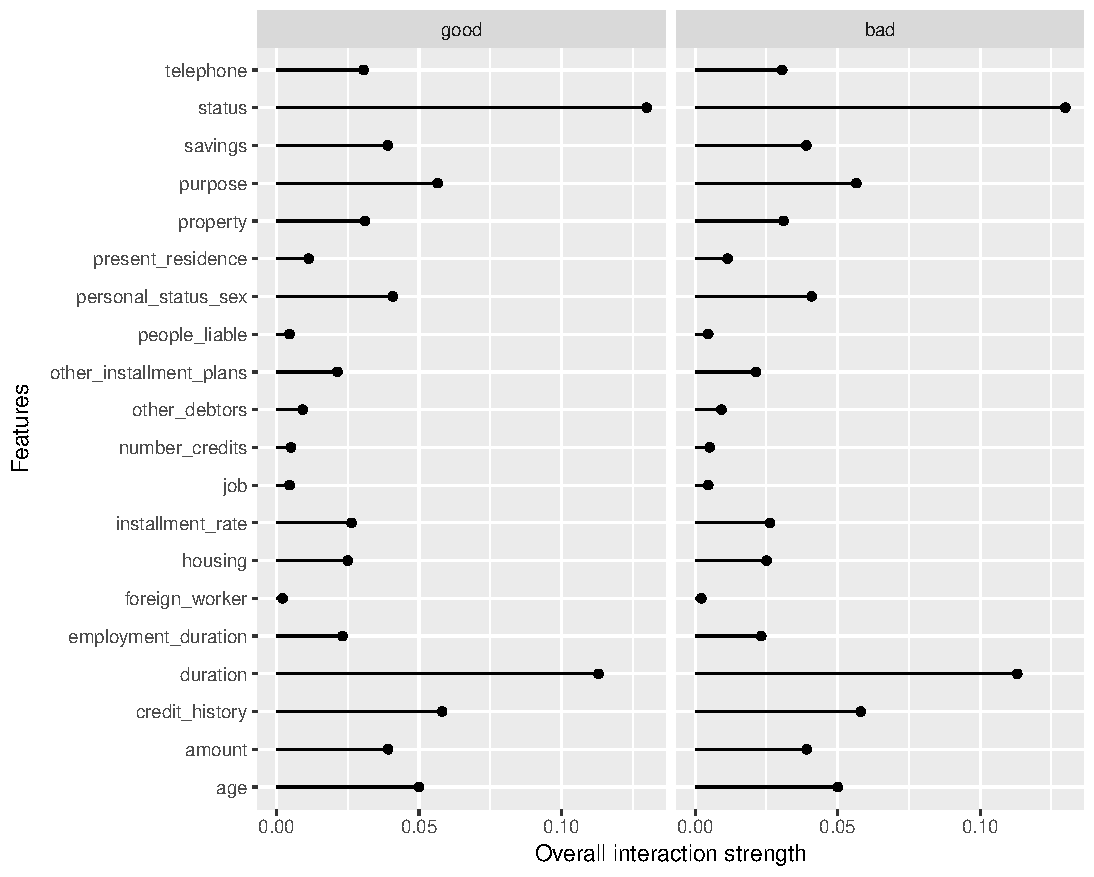
\includegraphics[width=0.8\linewidth]{plots/interaction} 

}

\caption{Interaction Strength (H-Statistic) between each feature and all other features}\label{fig:interaction}
\end{figure}

\begin{enumerate}
\def\labelenumi{\arabic{enumi}.}
\setcounter{enumi}{7}
\item
  Does having no \texttt{property} mean bad \texttt{credit\_risk} and how does this relate to age\\
  NaN
\item
  Being a foreign worker does not affect your credit risk. If this feature is important for prediction, this implies discrimination.\\
  As can be seen from Figure \ref(fig:feature-importance), \texttt{foreign\_worker} is the 6th least important feature in 20 features in total. Looking at the ALE plot for \texttt{foreign\_worker} in Figure \ref(fig:ale-foreign-worker), we notice a strange phenomenon. If you are a foreign worker, it brings positive effect to your credit, and otherwise, a slight negative effect. However, this can be explained by the distribution of the feature (Figure \ref(fig:geom-bar-foreign-worker)). The proportion of foreign workers is less than 4\% the proportion of native workers (37 to 963) and almost 90\% of the foreign workers in the dataset has good credit however only about 70\% of the native workers in the dataset has good credit.
\end{enumerate}

\begin{Shaded}
\begin{Highlighting}[]
\KeywordTok{summary}\NormalTok{(data}\OperatorTok{$}\NormalTok{foreign_worker)}
\end{Highlighting}
\end{Shaded}

\begin{verbatim}
## yes  no 
##  37 963
\end{verbatim}

\begin{Shaded}
\begin{Highlighting}[]
\NormalTok{eff <-}\StringTok{ }\NormalTok{FeatureEffect}\OperatorTok{$}\KeywordTok{new}\NormalTok{(model, }\DataTypeTok{feature =} \KeywordTok{c}\NormalTok{(}\StringTok{"foreign_worker"}\NormalTok{))}
\NormalTok{eff}\OperatorTok{$}\KeywordTok{plot}\NormalTok{()}
\end{Highlighting}
\end{Shaded}

\textbackslash begin\{figure\}

\{\centering 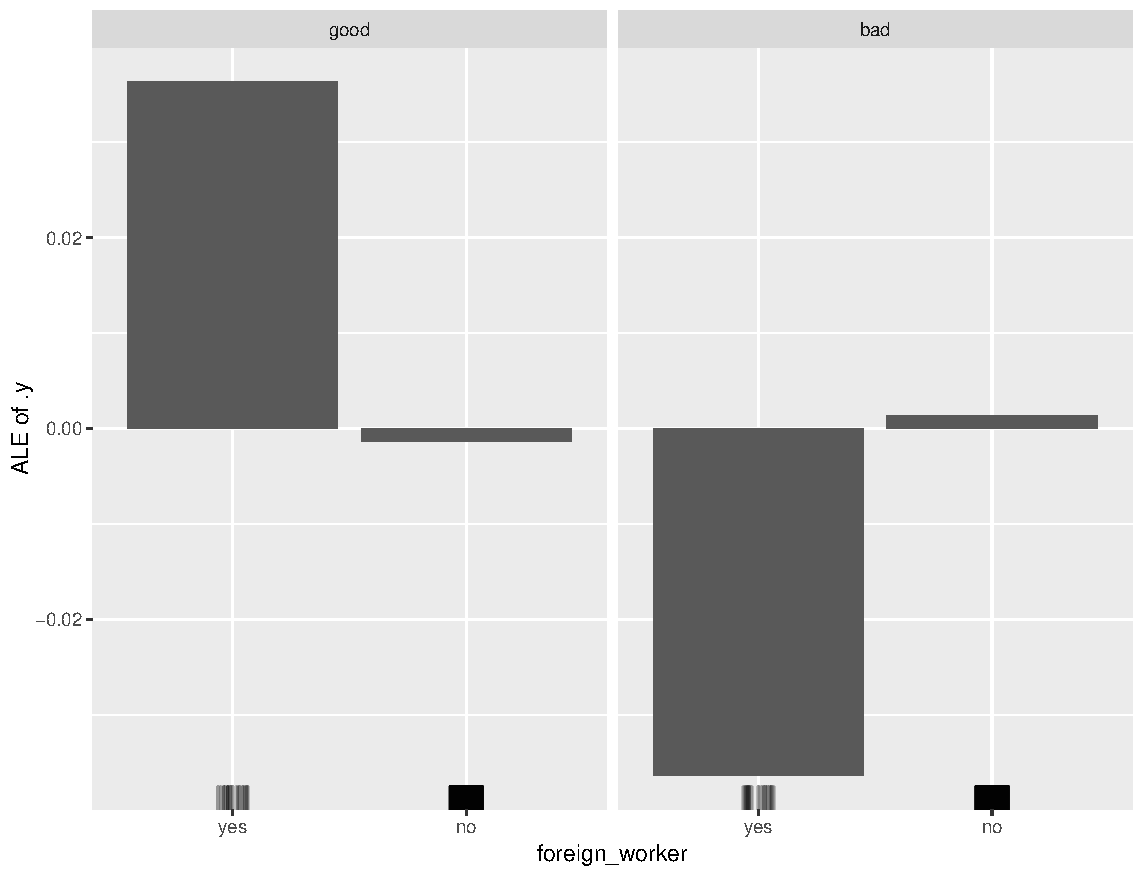
\includegraphics[width=0.8\linewidth]{plots/ale_foreign_worker}

\}

\textbackslash caption\{ALE Plot for \texttt{foreign\_worker}\}\label{fig:ale-foreign-worker}
\textbackslash end\{figure\}

\begin{Shaded}
\begin{Highlighting}[]
\KeywordTok{ggplot}\NormalTok{(}\DataTypeTok{data =}\NormalTok{ data, }\DataTypeTok{mapping =} \KeywordTok{aes}\NormalTok{(}\DataTypeTok{x =}\NormalTok{ foreign_worker, }\DataTypeTok{fill =}\NormalTok{ credit_risk)) }\OperatorTok{+}\StringTok{ }\KeywordTok{geom_bar}\NormalTok{()}
\end{Highlighting}
\end{Shaded}

\textbackslash begin\{figure\}

\{\centering 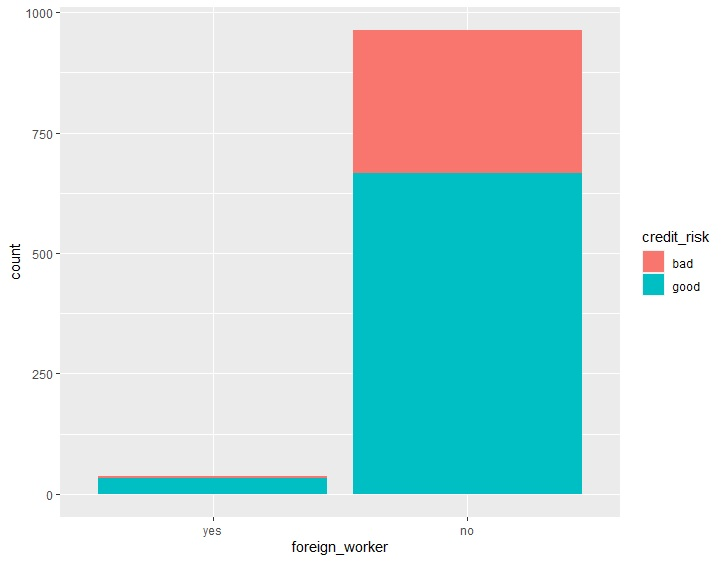
\includegraphics[width=0.8\linewidth]{plots/geom_bar_foreign_worker}

\}

\textbackslash caption\{Bar Plot for \texttt{foreign\_worker} with distribution of \texttt{credit\_risk} in each level\}\label{fig:geom-bar-foreign-worker}
\textbackslash end\{figure\}

\begin{enumerate}
\def\labelenumi{\arabic{enumi}.}
\setcounter{enumi}{9}
\tightlist
\item
  The better the savings, the better your credit risk\\
  We continue to use ALE plot to answer this question. Looking at the plot in Figure \ref(fig:ale-savings), it is clear that the more money for savings, the more positive effect it has on your credit risk. And if there is no savings account, the credit can suffer.
\end{enumerate}

\begin{Shaded}
\begin{Highlighting}[]
\NormalTok{eff <-}\StringTok{ }\NormalTok{FeatureEffect}\OperatorTok{$}\KeywordTok{new}\NormalTok{(model, }\DataTypeTok{feature =} \KeywordTok{c}\NormalTok{(}\StringTok{"savings"}\NormalTok{))}
\NormalTok{eff}\OperatorTok{$}\KeywordTok{plot}\NormalTok{()}
\end{Highlighting}
\end{Shaded}

\begin{figure}

{\centering 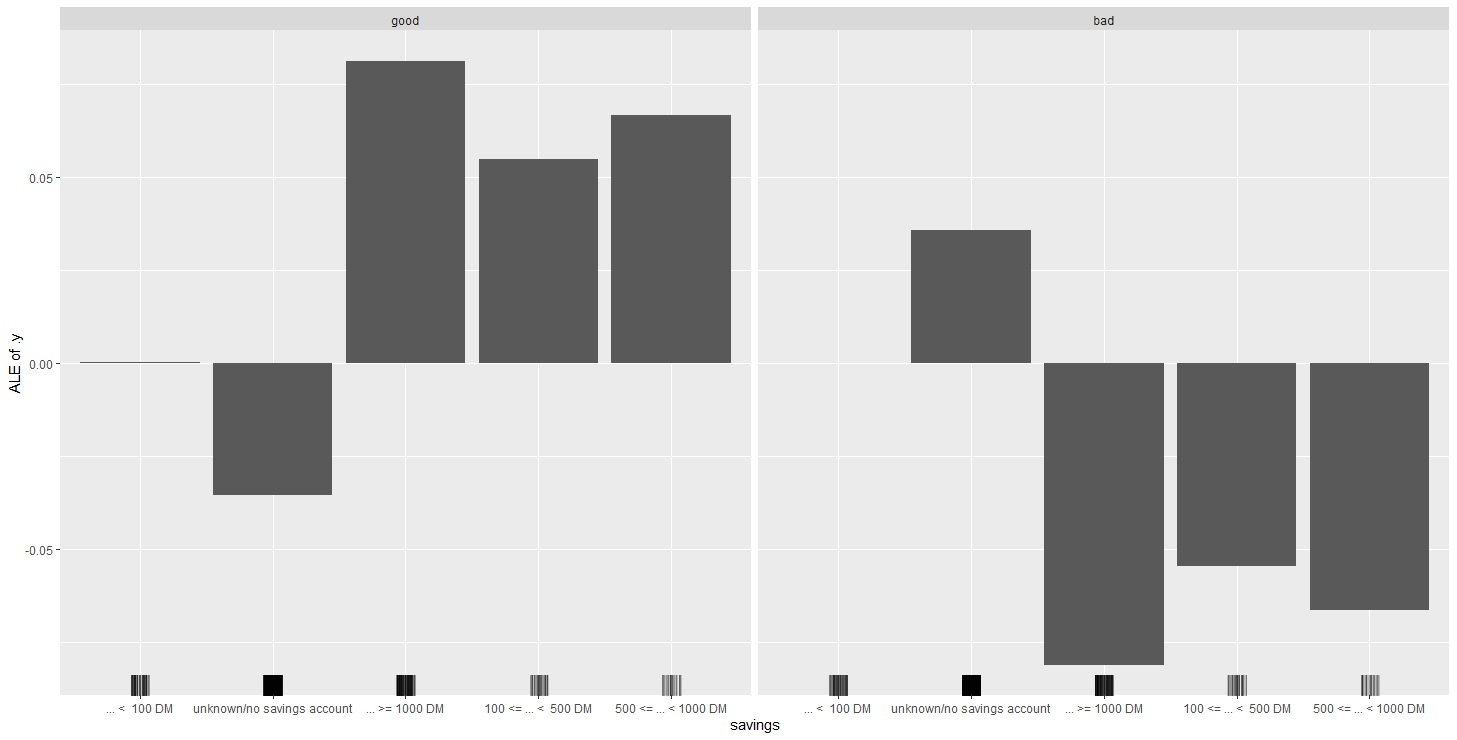
\includegraphics[width=0.8\linewidth]{plots/ale_savings} 

}

\caption{ALE Plot for `savings`}\label{fig:ale-savings}
\end{figure}

\begin{enumerate}
\def\labelenumi{\arabic{enumi}.}
\setcounter{enumi}{10}
\item
  The higher the \texttt{installment\_rate} the better the \texttt{credit\_risk}\\
  NaN
\item
  Does owning a house (\texttt{housing}) mean good \texttt{credit\_risk}\\
  NaN
\end{enumerate}

\end{document}
